\documentclass{article}

\usepackage{minted, graphicx, enumerate}
\graphicspath{{./}}
\title{VHDL Lab2 Report}
\date{\today}
\author{JHIH-SIOU LI, 105021226}


\begin{document}
	\maketitle
	\pagebreak
	\section{Design Chart}
		\t Here is my design chart synthesized by using Design Vision.\\
		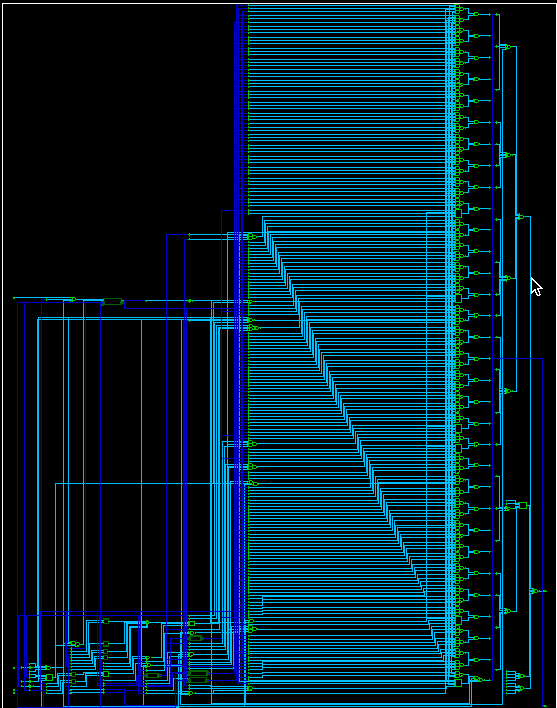
\includegraphics{design_chart.png}
	\section{Some other charts and descriptions}
		\t Since this time we don't need to build the circuit from drawing a K-Map, it is far more easier to build a ALU.\\
		For the logic gate part, I just need to write down the sum of products and make it by stacking up the NAND gate (like this):
		\begin{minted}[frame=lines, framesep=4mm, autogobble]{vhdl}
			module AND (a, b, c);
				input  a, b;
				output c;
				wire nand_0;
				// IMPLEMENTATION
				nand nand1(nand_0, a, b);
				NOT N1(nand_0, c);
			endmodule

			module OR (a, b, c);
				input  a, b;
				output c;
				wire not_0, not_1;
				// IMPLEMENTATION
				NOT N1(a, not_0);
				NOT N2(b, not_1);
				nand(c, not_0, not_1);
			endmodule

			module NOT (a, b);
				input  a;
				output b;
				// IMPLEMENTATION
				nand(b, a, a);
			endmodule
	
		\end{minted}
		Once we got these basic logic gates done by using NAND gate, we can then use them to build up more complex gates such as NOR, XOR, XNOR gates.\\
		Here are the truth tables:\\
		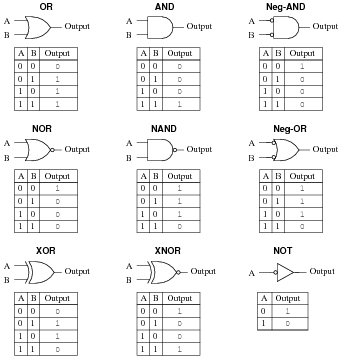
\includegraphics[width=8cm]{truth-table1.png}

		Since the Lab2 didn't require us to draw the K-Maps, I'm going to ommit them here.

	\section{Problems}
		\t The main problem in my Verilog design were 2 important errors:
		\begin{enumerate}
			\item{Putting another always block inside a always block.\\ This caused me to seriously delayed the progress of this assignment for few days and I had no clue about what is going wrong.}
			\item{Wrong array size in my wire variables.\\ With this typo, I spent about 3 hrs to find the error in my Decoder and Arbiter and found nothing.(here)
				\begin{minted}[frame=lines, framesep=4mm, autogobble]{vhdl}
					wire [32-1:0]  dec_1;
					wire [5-1:0] arb_1;
					...
					4'b1110: Y = dec_1; 
					4'b1111: Y = arb_1;
				\end{minted}
				If we assign the input with the size that is too small, then it will fill up Y's remaining blanks with 'z's, which is not our desired '0's.}

		\end{enumerate}
		To sum it up, it was nothing but careless typos and conceptual inaccurarcy.

	\section{Simulation Outcome}
		\t Here is my simulation outcome of ncverilog:\\
		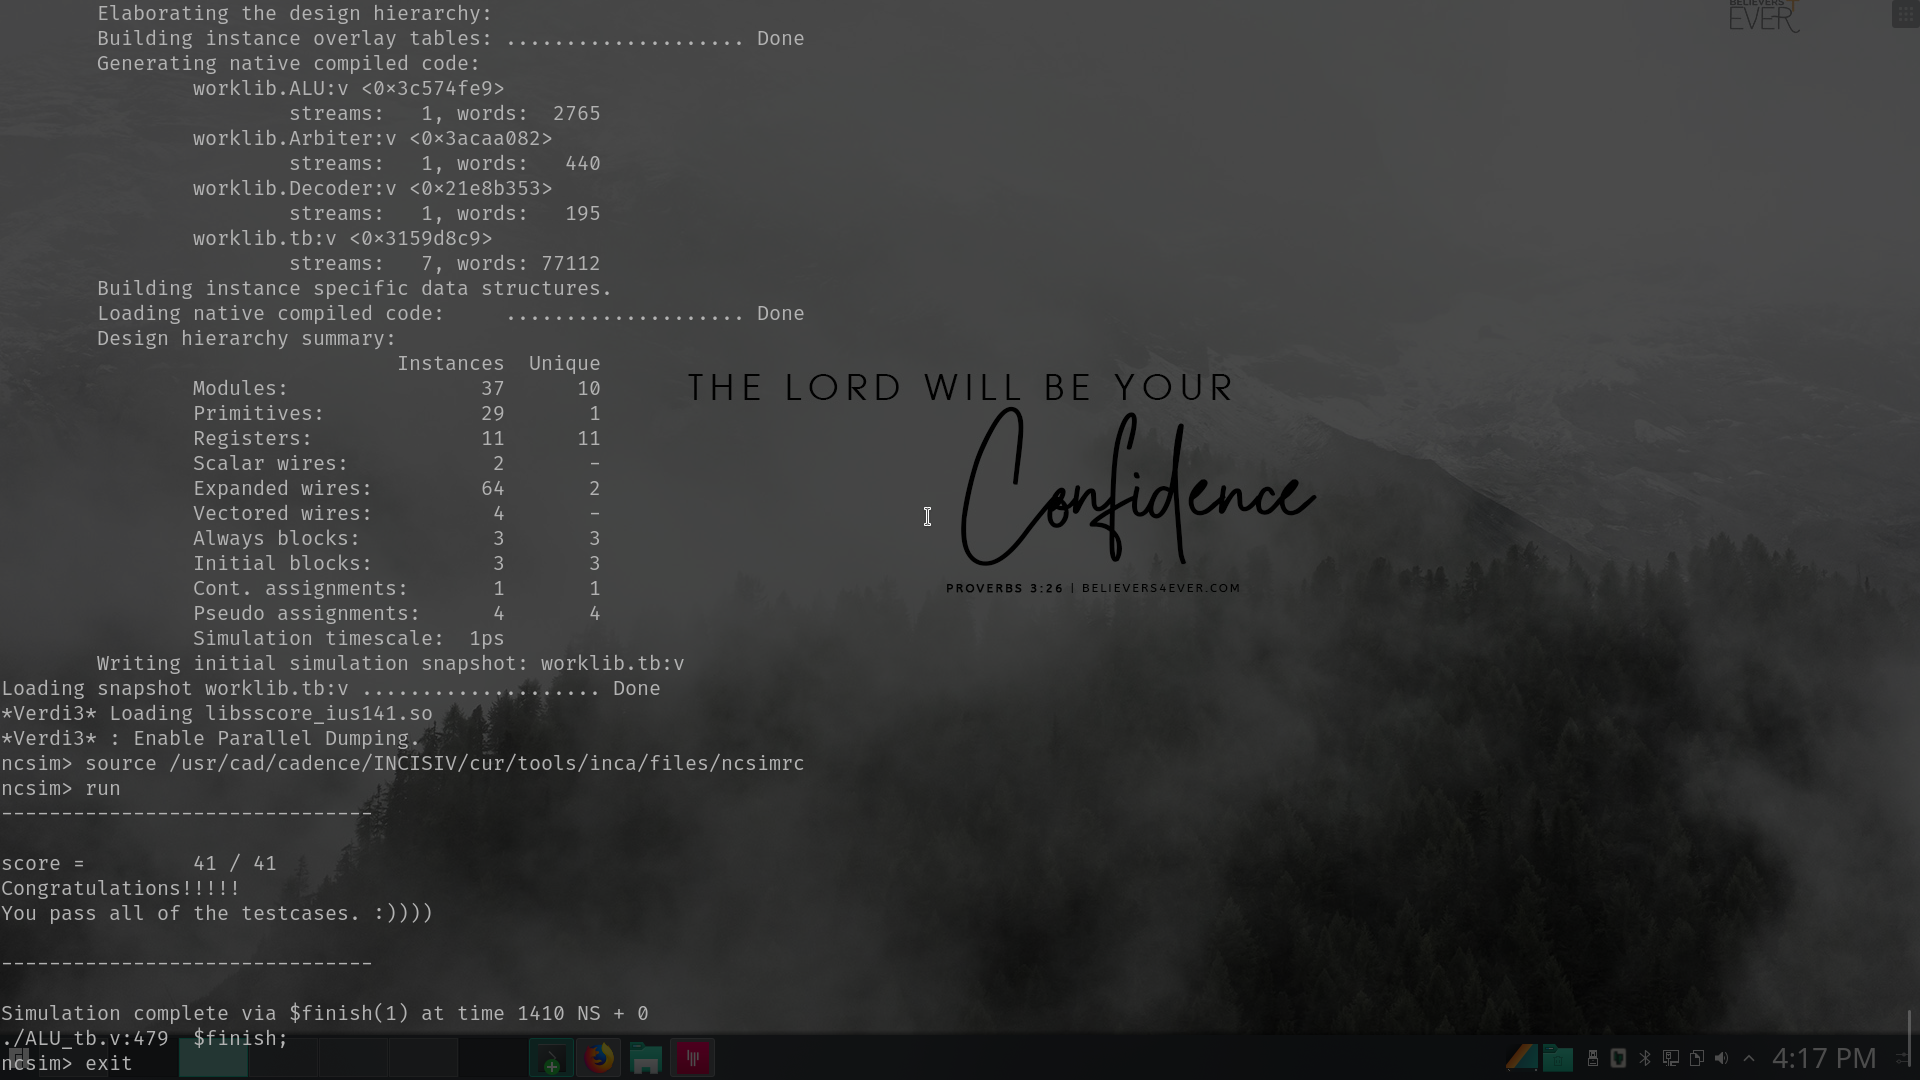
\includegraphics[width = 16cm]{sim_outcome.png}
	\section{Report Area}
		\t The content inside my report area txt file.\\
		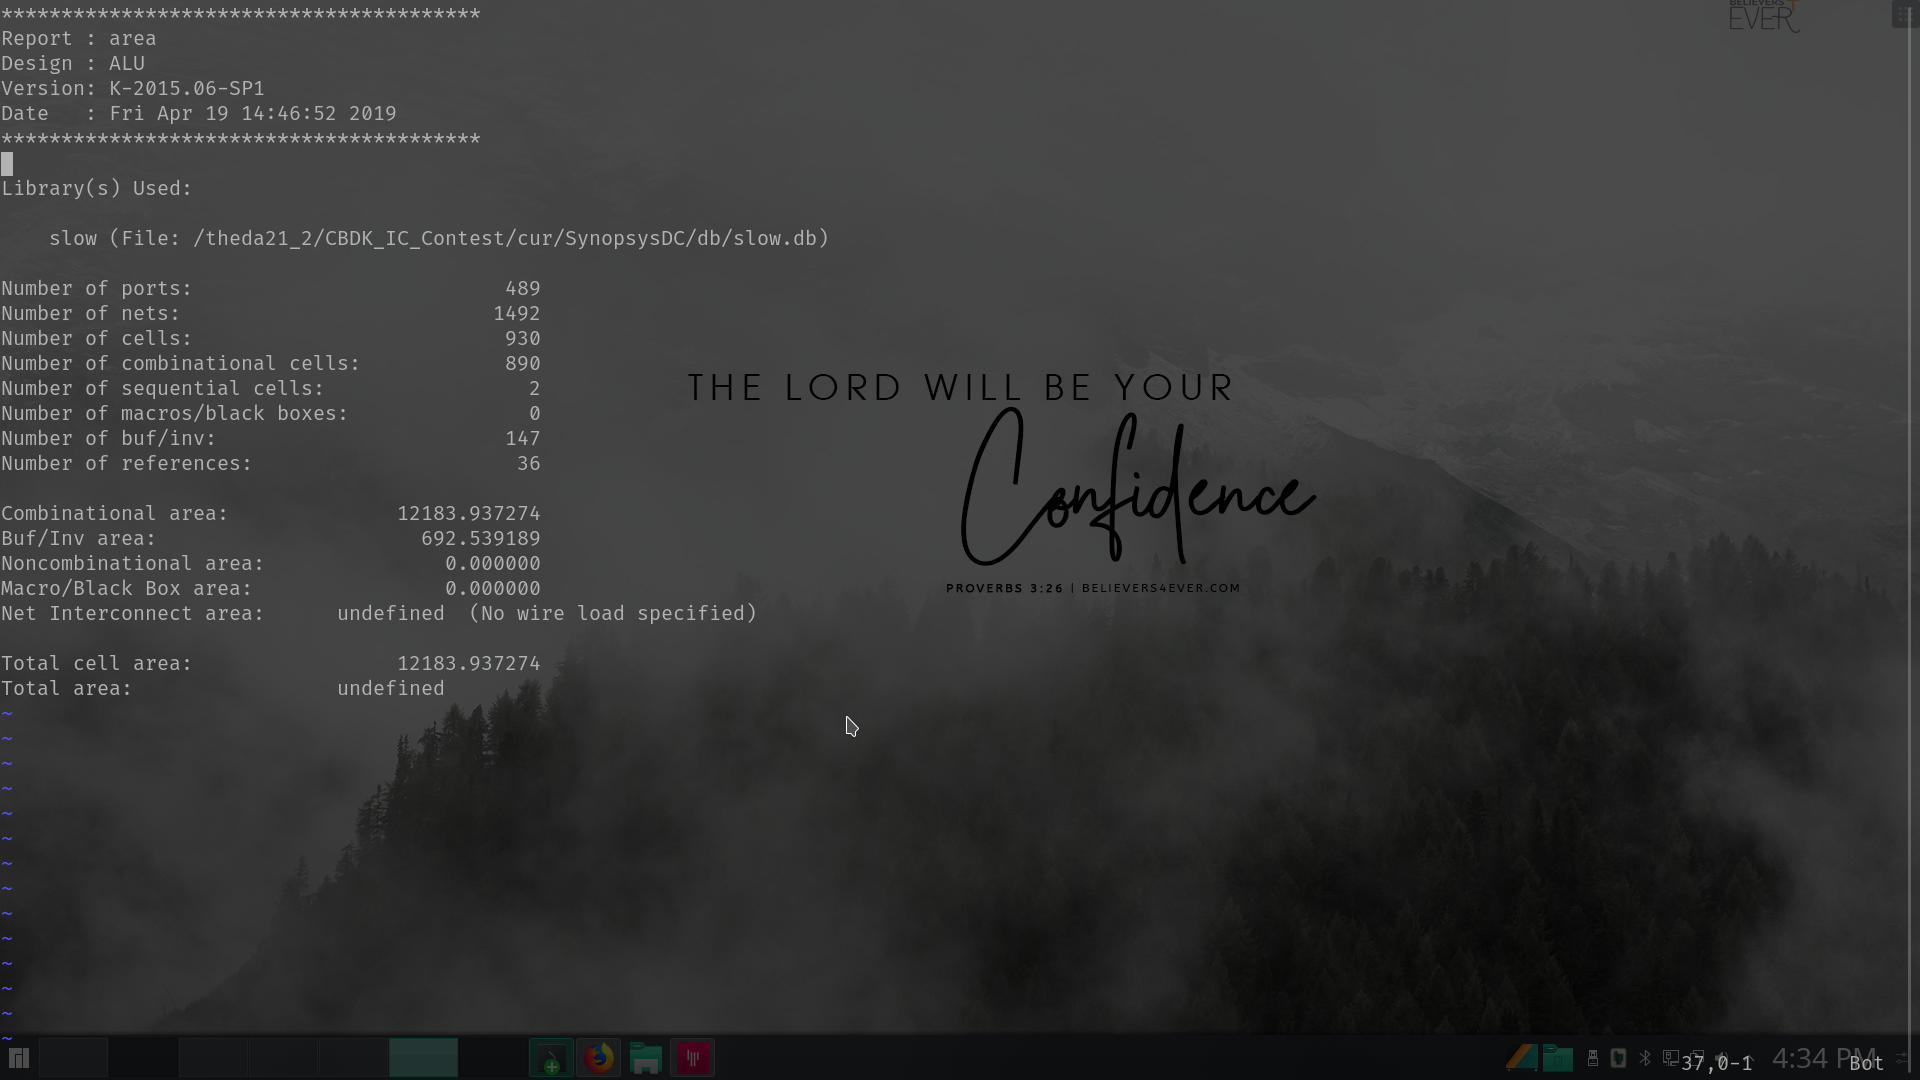
\includegraphics[width = 16cm]{report_area1.png}

\end{document}
